\begin{problem}{Just the Last Digit}{standard input}{standard output}{2 seconds}{512 megabytes}

Jessie has recently started jogging and tracking the progress with a fitness band. There are $n$ spectacular spots on a nearby hill. As running uphill is hard for an amateur jogger, Jessie is only going to run downhill. The spots have numbers from $1$ to $n$, the higher the number is, the lower the spot is. Some pairs of spots are connected by trails, and for our purpose, we will only consider trails $i \to j$ going from a higher spot to a lower spot ($i < j$).

\begin{center}
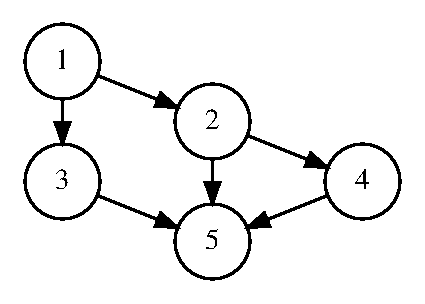
\includegraphics[bb=0 0 188 130]{graph.eps}
\end{center}

Jessie successfully finished some number of jogs, running through each possible sequence of spots, for which a trail between any two consecutive spots exists, exactly once.
Now Jessie is planning to restore the map of all trails with the help of data collected by the fitness band. Unfortunately, the display on the band is small, and can only show the last digit of the number of jogs Jessie did between each pair of spots $i$ and $j$ where $1 \le i < j \le n$. Can you help Jessie restore the map of the hill given this data?

 

\InputFile
The first line of the input contains an integer $n$~--- the number of spots on the hill  ($2 \le n \le 500$).
Next, $n$ lines follow: the $i$-th line contains $n$ characters $a_{i,1}, a_{i,2}, \ldots, a_{i,n}$. Character $a_{i, j}$ is the last digit of the number of different jogs made by Jessie starting at the $i$-th spot and ending at the $j$-th spot. For every $i \ge j$, $a_{i, j} = 0$.

It is guaranteed that a solution always exists for the given input data.

\OutputFile
Print $n$ lines, describing the map of the hill in the similar format: the $i$-th line should contain $n$ characters, where $j$-th character is \t{1} if there is a trail from the $i$-th spot to the $j$-th spot, and \t{0} otherwise. For every $i \ge j$, the $j$-th character in the $i$-th row must be \t{0}.

\Example

\begin{example}
\exmpfile{example.01}{example.01.a}%
\end{example}

\end{problem}

